\documentclass{beamer}  
\usetheme{CambridgeUS}  
% \usepackage{pgfpages}
\usepackage{color}
\usepackage{xeCJK}
% \usepackage{minted}
\usepackage{subfigure}
\usepackage{amsmath}
\usepackage{algorithm}
\usepackage{algorithmic}

\newtheorem{Def}{Definition}
\newtheorem{Theo}{Theorem} 

% \usepackage{fontspec}  
% \setsansfont{楷体} % font name is case-sensitive  
\setCJKsansfont{楷体}
% \setbeameroption{show notes on second screen}

\newcommand{\hl}[1]{{\color{blue}{#1}}}

\begin{document}

\title{独立成分分析(ICA)}
\author{余海涛 1732985}
\frame{\titlepage}


%%%%%%%%%%%%%%%%%%%%%%%%%%%%%%%%%%%%%%
\begin{frame}{独立成分分析}  
   独立成分分析(Independent Components Analysis, ICA)是一种利用\hl{统计原理}进行计算的方法,它是一个\hl{线性变换},这个变换把数据或信号分离成\hl{统计独立}的\hl{非高斯}的信号源。\footnote{Wikipedia}
    \note{这是一个注释}
\end{frame}  

%%%%%%%%%%%%%%%%%%%%%%
\begin{frame}{鸡尾酒会问题}
    假设你在一个房间里,有三个人在同时讲话,还有三个麦克风,摆放在不同的位置进行录音,麦克风记录下的三个信号可以表示为$x_1(t)$,$x_2(t)$和$x_3(t)$,可以认为每一个信号都是三个讲话者发出的信号的加权和,假设三个讲话者的信号用$s_1(t)$,$s_2(t)$和$s_3(t)$表示,则$x_i$和$s_i$的关系表示为
    \begin{equation}
    \left\{
    \begin{aligned}
    x_1(t)=a_{11}s_1(t)+a_{12}s_2(t)+a_{13}s_3(t) \\
    x_2(t)=a_{21}s_1(t)+a_{22}s_2(t)+a_{23}s_3(t) \\
    x_3(t)=a_{31}s_1(t)+a_{32}s_2(t)+a_{33}s_3(t)
    \end{aligned}
    \right.
    \end{equation}
    {\color{red}注意,模型忽略了录音的时延和其他影响因素,假设三个录音机的采样是同步的}
\end{frame}

%%%%%%%%%%%%%%%%%%%%%%
\begin{frame}{问题定义}
    假设观察到$n$个随机变量$x_1,x_2,\ldots,x_n$,而这些变量是由另外$n$个随机变量$s_1,s_2,\ldots,s_n$线性组合得到,可以用矩阵形式表示如下
    \begin{equation}
    \mathbf{x}=\mathbf{As}
    \end{equation}
    其中
    \begin{equation}
    \mathbf{x}=\left(
    \begin{aligned}
    x_1\\
    x_2\\
    \vdots\\
    x_n
    \end{aligned}
    \right),
    \mathbf{s}=\left(
    \begin{aligned}
    s_1\\
    s_2\\
    \vdots\\
    s_n
    \end{aligned}
    \right),
    \mathbf{A}=\left(
    \begin{array}{cccc}
    a_{11} & a_{12} & \cdots & a_{1n} \\ 
    a_{21} & a_{22} & \cdots & a_{2n} \\ 
    \vdots & \vdots & \ddots & \vdots \\ 
    a_{n1} & a_{n2} & \cdots & a_{nn}
    \end{array} 
    \right)
    \end{equation}
    已知$\mathbf{x}$的统计数据,要求估计$\mathbf{A}$的值,以得到$s$原始信号
\end{frame}


%%%%%%%%%%%%%%%%%%%%%%
\begin{frame}{假设和不确定性}
    为了确保ICA模型可以被估计,必须做出下面的假设和约束
    \begin{enumerate}
        \item 假设原始信号是统计独立的
        \item 独立成分具有非高斯的分布
        \item 未知的混合矩阵是方阵
    \end{enumerate}
    
    ICA模型中存在下面一些不确定性
    \begin{enumerate}
        \item 无法确定独立成分的方差
        \item 无法确定独立成分的次序
    \end{enumerate}
\end{frame}

\begin{frame}{关于非高斯性}
\begin{figure}[h]
    \centering
    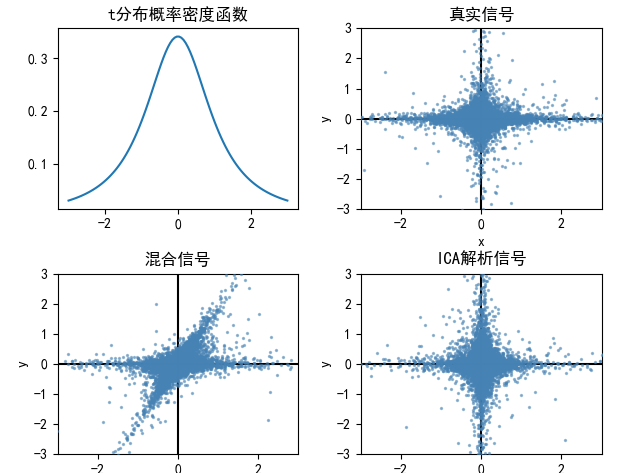
\includegraphics[width=0.6\linewidth]{figs/t-dist.png}
    \caption{两个独立的t分布}
    \label{fig:t_dist}
\end{figure}
\end{frame}

\begin{frame}{关于非高斯性}
\begin{figure}[h]
    \centering
    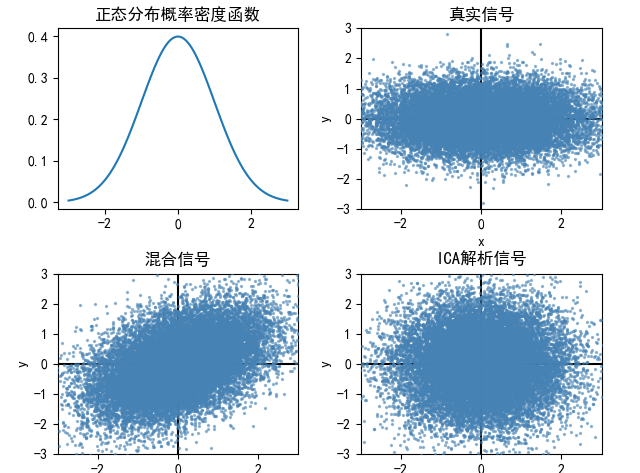
\includegraphics[width=0.6\linewidth]{figs/normal-dist.png}
    \caption{两个独立的正态分布}
    \label{fig:normal_dist}
\end{figure}
\end{frame}

%%%%%%%%%%%%%%%%%%%%%%
\begin{frame}{极大化非高斯性的原理}
由中心极限定理可以得到,独立的随机变量之和的分布趋向于高斯分布。或者不那么严格的讲,可以认为两个独立随机变量之和形成的分布比两个原始的随机变量中的任意一个更接近于高斯分布。

现在为了估计出ICA数据模型中的一个独立成分,可以考虑对$x_i$进行某种线性组合,有:
\begin{equation}
y=\mathbf{b}^T\mathbf{x}=\mathbf{q}^T\mathbf{s}=\sum_{i}q_is_i
\end{equation}

问题在于:我们如何使用中心极限定理确定$\mathbf{b}$,使它刚好等于$\mathbf{A}$的逆矩阵中的一行?

我们可以通过改变$\mathbf{q}$中的系数来观察$y=\mathbf{q}^T\mathbf{s}$的分布如何变化。这里的基本思想是,既然两个独立随机变量之和分布的高斯性都比原始变量的更强,那么$y=\mathbf{q}^T\mathbf{s}$应该比任意一个$s_i$的高斯性更强。
\end{frame}

%%%%%%%%%%%%%%%%%%%%%%
\begin{frame}{度量非高斯性}
基于峭度(峰度)\footnote{式子中所有随机变量都假定是零均值的}:

\begin{equation}
kurt(y)=E\{y^4\}-3(E\{y^2\})^2
\end{equation}

基于负熵:

\begin{align}
H(y)&=-\int \, p_y(y)\mathrm{log}p_y(y)\,\mathrm{d}y\\
J(y)&=H(y_{gauss})-H(y)\\
            &\approx \frac{1}{12}E\{y^3\}^2+\frac{1}{48}\mathrm{kurt}(y)^2
\end{align}

其中$y_{gauss}$是与$y$具有相同相关和协方差矩阵的高斯随机变量

\note{极大似然估计方法,高斯变量具有最大的熵}
\end{frame}


%%%%%%%%%%%%%%%%%%%%%%
\begin{frame}{不动点迭代}
\begin{Def}{不动点}
    对于给定的函数$\varphi$,如果一个数$x$满足$\varphi(x)=x$,则这个数是一个不动点
\end{Def}


%\begin{figure}[h]
%    \centering
%    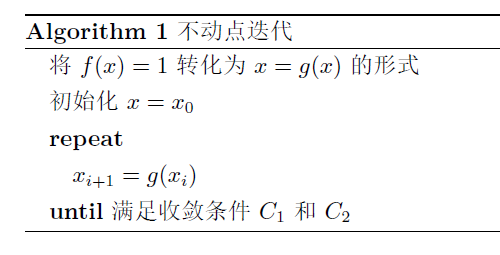
\includegraphics[width=0.6\linewidth]{figs/alg.png}
%    \label{alg}
%\end{figure}
%\begin{algorithm}
%    \caption{不动点迭代}  
%    \label{alg:apxB}
%    \begin{algorithmic}  
%        \STATE {将$f(x)=1$转化为$x=g(x)$的形式}
%        \STATE {初始化$x=x_0$}   
%        \REPEAT
%        \STATE $x_{i+1}=g(x_i)$
%        \UNTIL {满足收敛条件$C_1$和$C_2$} 
%    \end{algorithmic}  
%\end{algorithm}

\begin{Theo}{不动点的收敛性定理}
    \label{theo:apxB}
    设迭代函数$\varphi(x)$在$[a,b]$上连续,且满足
    
    $C_1$\ 当$x\in [a,b]$时,$a\leq\varphi(x)\leq b$;
    
    $C_2$\ 存在正数$L$,满足$0<L<1$,且$\forall x\in [a,b]$,有$|\varphi '|\leq L$
    
    则有,
    
    1. 方程$x=\varphi(x)$在$[a,b]$内有唯一解$x^*$
    
    2. 对于任意初值$x_0\in [a,b]$,迭代法均收敛于$x^*$
    
    3. $|x_k-x^*|\leq \frac{L}{1-L}| x_k-x_{k-1} |$
    
    4. $|x_k-x^*|\leq \frac{L^k}{1-L}| x_1-x_0 |$
\end{Theo}
\end{frame}


%%%%%%%%%%%%%%%%%%%%%%
\begin{frame}{FastICA算法}
\begin{table}[h]
    \centering 
    \begin{tabular}{p{0.8\columnwidth}}
        \hline 
        1. 对数据进行中心化使其均值为0\\
        2. 然后对数据进行白化得到$z$\\
        3. 选择要估计的独立成分个数$m$\\
        4. 初始化所有的$\mathbf{w}_i,i=1,2,\cdots,m$,其中每个$\mathbf{w}_i$都具有单位范数。用下面第6步的方法对矩阵$\mathbf{W}$进行正交化\\
        5. 对每一个$i=1,2,\cdots,m$,更新$\mathbf{w}_i$:$\mathbf{w}_i\leftarrow E\{ \mathbf{z} g(\mathbf{w}_i^T\mathbf{z}) \}-E\{ g'(\mathbf{w}_i^T\mathbf{z}) \}\mathbf{w}_i$,其中g的形式可以取$g_1(y)=tanh(a_1y)$或$g_2(y)=y\,exp(-y^2/2)$或$g_3(y)=y^3$\\
        6. 对矩阵$\mathbf{W}=(\mathbf{w_1},\cdots,\mathbf{w_n})^T$进行正交化:$\mathbf{W}\leftarrow(\mathbf{WW}^T)^{-1/2}\mathbf{W}$\\
        7. 如果没有收敛,则返回步骤5\\
        \hline
    \end{tabular}
    \caption{估计多个独立成分的FastICA算法,使用对称正交化方法。实际应用中,期望用样本的平均值来估计}
    \label{fast_ica_alg}
\end{table}
\end{frame}


%%%%%%%%%%%%%%%%%%%%%%
\begin{frame}{白化}
    白化性(whiteness)是指一个零均值的随机向$y$的各个分量具有相同的单位方差且互相不相关,换句话说$y$的协方差矩阵是单位矩阵:
    \begin{equation}
    E\{\textbf{yy}^T\}=\mathbf{\mathit{I}}
    \end{equation}
    白化意味着我们将观察得到的数据向量$\mathbf{x}$与某个矩阵$\mathbf{V}$相乘后得到的是一个新的白化的向量:
    \begin{equation}
    \mathbf{z}=\mathbf{Vx}
    \end{equation}
    白化变换总是可实现的,一般可以利用协方差矩阵的特征值分解(EVD)。
\end{frame}

%%%%%%%%%%%%%%%%%%%%%%
\begin{frame}{实际应用}
\begin{figure}[h]
    \centering
    \includegraphics[width=0.9\linewidth]{figs/result1}
    \caption{无高斯噪声情况下的ICA分离结果}
    \label{fig:result1}
\end{figure}
\end{frame}

%%%%%%%%%%%%%%%%%%%%%%
\begin{frame}{实际应用}
\begin{figure}[h]
    \centering
    \includegraphics[width=0.9\linewidth]{figs/result2}
    \caption{有高斯噪声情况下的ICA分离结果}
    \label{fig:result2}
\end{figure}
\end{frame}

\begin{frame}{实际应用}
\begin{figure}[h]
    \centering
    \subfigure[原始人脸]{
        \label{fig:face0}
        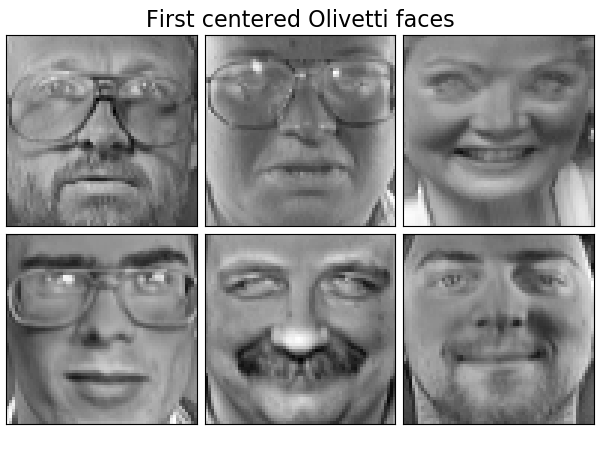
\includegraphics[width=1.2in]{figs/face0.png}
    }
    \hspace{0.2in}
    \subfigure[PCA降维]{
        \label{fig:face1}
        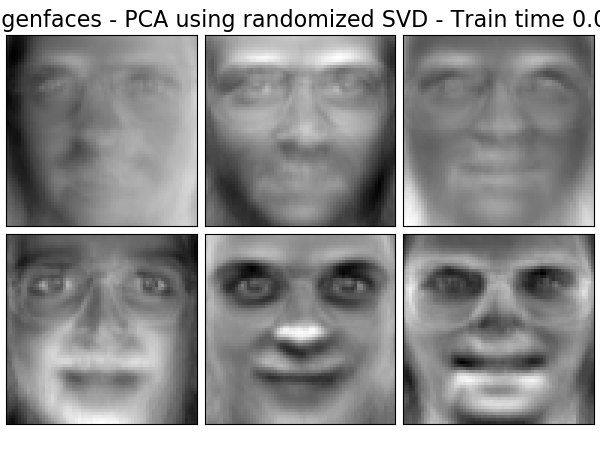
\includegraphics[width=1.2in]{figs/face1.png}
    }
    \hspace{0.2in}
    \subfigure[ICA降维]{
        \label{fig:face2}
        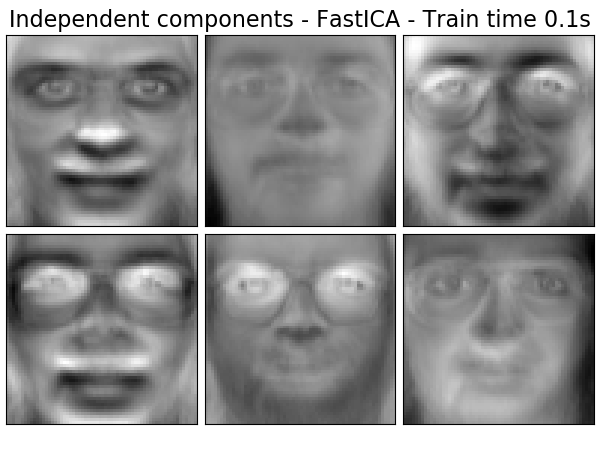
\includegraphics[width=1.2in]{figs/face2.png}
    }
    \caption{人脸图像降维示例}
    \label{fig:face}
\end{figure}
\end{frame}

%%%%%%%%%%%%%%%%%%%%%%
\begin{frame}{续}
    \[
        \left\{
            \begin{aligned}
                Music_{left} &= BGM_{left} + Voice\\
                Music_{right}&= BGM_{right} + Voice\\
            \end{aligned}
        \right.
    \]
%    \begin{figure}[h]
%        \centering
%        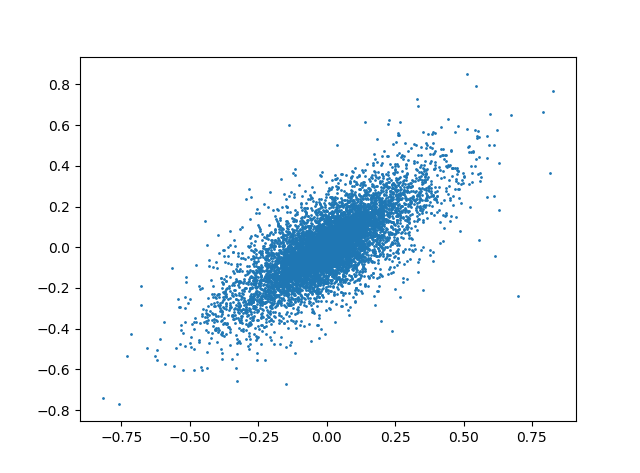
\includegraphics[width=0.5\linewidth]{figs/lz.png}
%        \caption{一首音乐左右声道}
%        \label{fig:music}
%    \end{figure}

\begin{figure}[h]
    \centering
    \subfigure[正常音乐左右声道]{
        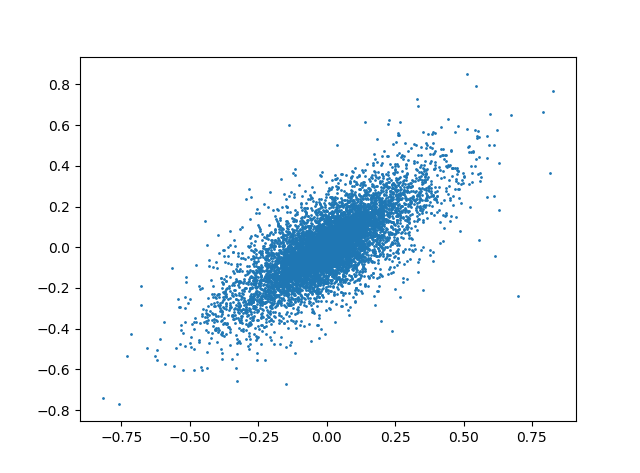
\includegraphics[width=1.5in]{figs/lz.png}
    }
    \hspace{0.2in}
    \subfigure[英语听力左右声道]{
        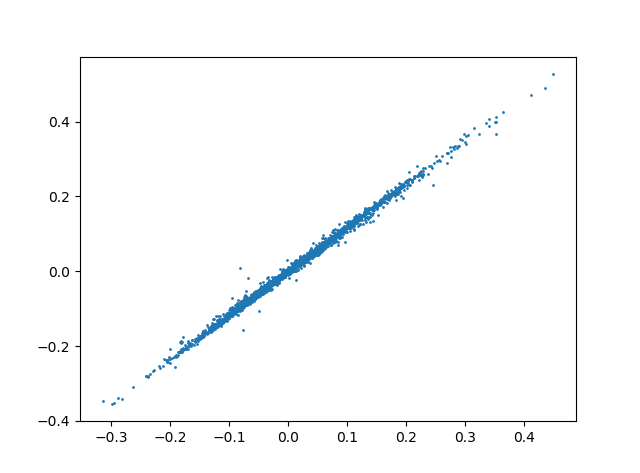
\includegraphics[width=1.5in]{figs/bbc.png}
    }
    \hspace{0.2in}
\end{figure}
\end{frame}

\begin{frame}{续}
\begin{figure}[h]
    \centering
    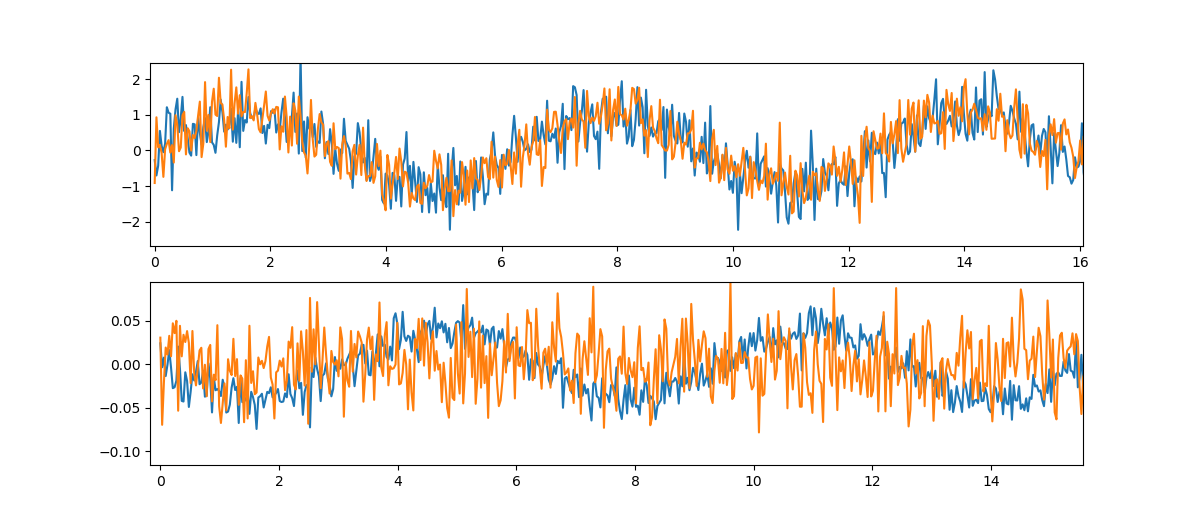
\includegraphics[width=0.9\linewidth]{figs/sin-rand.png}
    \caption{音乐双声道模拟}
\end{figure}
\end{frame}

\end{document}  